\entry{2026-10-18}{Priority 2: qualification, 2D accuracy--cost fronts, observed time order}

Lane \texttt{2026-10-18-jcp-qualify}, last commit \texttt{4399491eb}, mirror \texttt{fb9b137be}. 16 jobs (A100/H200, \texttt{jax\_backend=gpu}), 4.13 of 35 GPU-h, nothing deferred; final report audit READY. The frozen 2D front \texttt{runs/FRONT-2D.json} (commit \texttt{2374fafe1}) feeds the 2D full-solver comparison. Numbers quoted from the generated \path{report.md}; errors are E0 conditional estimates.

\begin{itemize}
\item \textbf{Qualification (2D):} 98 of 112 configurations pass the solver (Q1) and quadrature (Q2) checks. LSPG-CN-R at $2\Delta t_0$ fails Q1 for R128 and R256 at every mesh (worst case 3.6--4.0e-4 vs bar 2.5e-4).
\item \textbf{Fronts (paired timing, one job per mesh):} the Galerkin CN scheme (registered as a diagnostic) holds 6 of 7 median-front places at every mesh; the most accurate member is R384 GAL-CN at $\Delta t_0$, 0.050\,\% median at 1.31$\times$ the reference cost (1.5$\times$ at $4096^2$). Primary comparisons keep the registered LSPG schemes; GAL-CN is reported separately.
\item \textbf{Observed time order:} LSPG-BE 1; GAL-CN 2; LSPG-CN-R 2 at R384 ($\hat p=1.96$) but 1.74 at R128 (no integer label). Valid over $\Delta t_0$ to $\Delta t_0/4$.
\item \textbf{Accuracy vs mesh, extended set:} 21 pass, 9 inconclusive (5 because a configuration is unqualified). \textbf{Accuracy vs $r$:} the 384$\to$512 regression recurs in every cell of the 128--512 range.
\item \textbf{3D quadrature (Q2):} only 4 of 55 tested speed3d configurations pass. Both speed3d H2 winners fail (successor-rule distance 8.1e-4 and 9.5e-4); coordinator coefficient-space recheck 0.94e-3 and 1.10e-3.
\end{itemize}
\begin{center}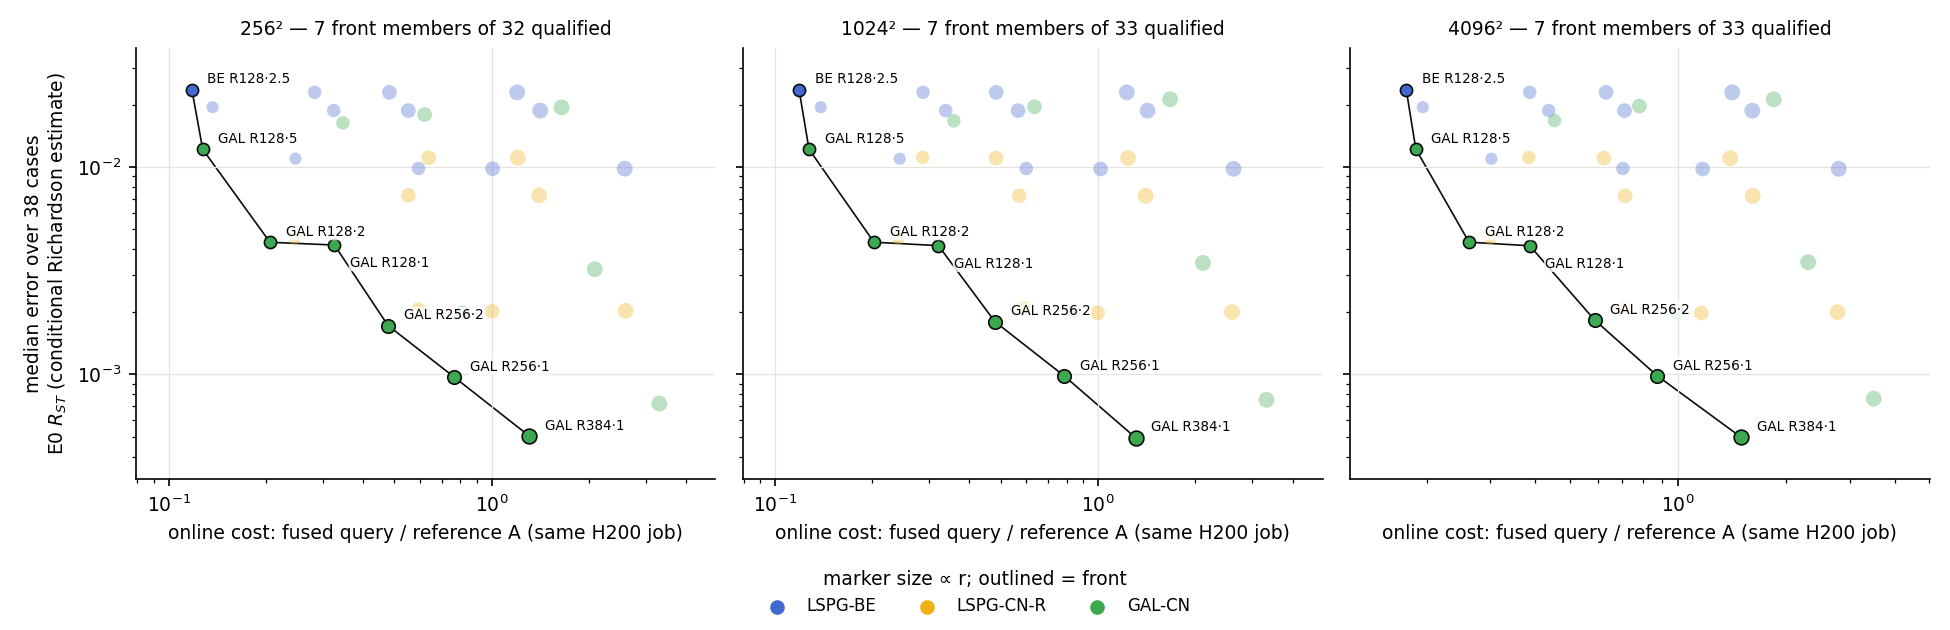
\includegraphics[width=0.48\linewidth]{figs/q_front2d_median.png}\hfill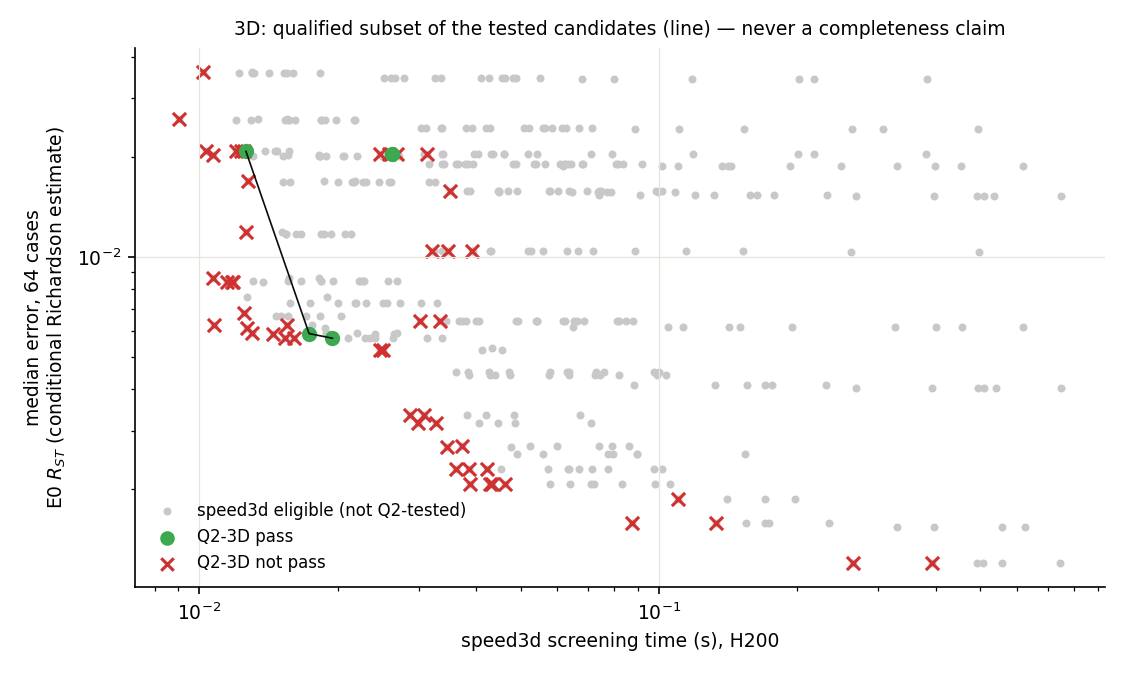
\includegraphics[width=0.48\linewidth]{figs/q_front3d.png}\end{center}

\subsection*{Corrections}
\retracted{The speed3d H2 speed-ups (2.01$\times$, 5.37$\times$, 17.2$\times$) are measured correctly but their winning configurations are \textbf{not quadrature-qualified}; they must not be called qualified. The combined lane's finalist table labels the R128 and R256-fallback ``fast equal accuracy'' arms (LSPG-CN-R at $2\Delta t_0$) qualified; under the every-case Q1 contract they are not. For Galerkin the stationarity ratio was replaced by a residual criterion (disclosed deviation).}
